\documentclass{article}

\usepackage[a4paper, total={6.75in, 8in}]{geometry}
\usepackage{amsmath}
\usepackage[document]{ragged2e}
\usepackage{listings}
\usepackage{multirow}
\usepackage{graphicx}
\usepackage{subcaption}
\usepackage{enumitem}

\usepackage{xcolor} 
\definecolor{vgreen}{RGB}{104,180,104}
\definecolor{vblue}{RGB}{49,49,255}
\definecolor{vorange}{RGB}{255,143,102}
\definecolor{vpurple}{RGB}{148,0,209}
\definecolor{vgray}{RGB}{245,245,245}

\lstdefinestyle{verilog}{
  language=verilog,
	backgroundcolor=\color{vgray},   
	commentstyle=\color{vgreen},
	keywordstyle=\color{vblue},
	numberstyle=\tiny\color{black},
	stringstyle=\color{vpurple},
	basicstyle=\scriptsize\ttfamily,
	breakatwhitespace=false,         
	breaklines=true,                 
	captionpos=t,                    
	keepspaces=true,                 
	numbers=left,                    
	numbersep=5pt,                  
	showspaces=false,                
	showstringspaces=false,
	showtabs=false,                  
	tabsize=2,
	language=Verilog,
	framesep=3mm
}

\begin{document}
\justify

\begin{center}
{\LARGE Xilinx Vivado IDE and the Arty A7 FPGA \par}
\end{center}

% \begin{center}
% {\large August 17, 2018 \par}
% \end{center}


\section*{Introduction}
This guide should get you up and running with Xilinx Vivado IDE (version 2018.2 at the time of writing). 
The target board used for this tutorial is the Arty A7-35T FPGA but you can still use this guide for other 
FPGA boards with little modifications.

\section*{Installation}
  \begin{enumerate}
    \item Download the Vivado webPack from Xilinx's website (https://www.xilinx.com/support/download.html). 
    You will need to create an account to download Vivado and also for generating a license key later on this tutorial.
    
    \item 
  \end{enumerate}

\section*{Creating a new project}
  \begin{enumerate}
    \item Launch the Vivado IDE. From the start page, select "Create Project".
    \item A dialog box (see Fig. \ref{fig:1-new_project_window}) will open describing the steps you will be taken to create a project. Click "Next" to continue.
      \begin{figure}[h!]
        \centering
        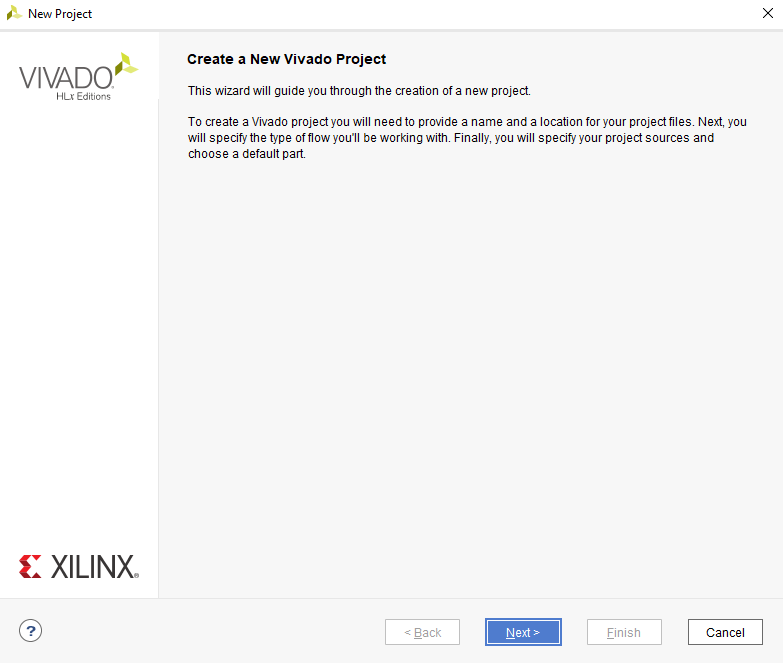
\includegraphics[width=0.5\linewidth]{img/program/1-new_project_window.png}
        \caption{New Project Window}
        \label{fig:1-new_project_window}
      \end{figure}

    \item The next step is to provide a name for the new project. Vivado will use this name when generating the project's folder structure. For this tutorial,
      set the name of the project as "updown\_counter" (see Fig. \ref{fig:2-project_name}). After setting the project's name, click "Next" to continue.
      \begin{figure}[h!]
        \centering
        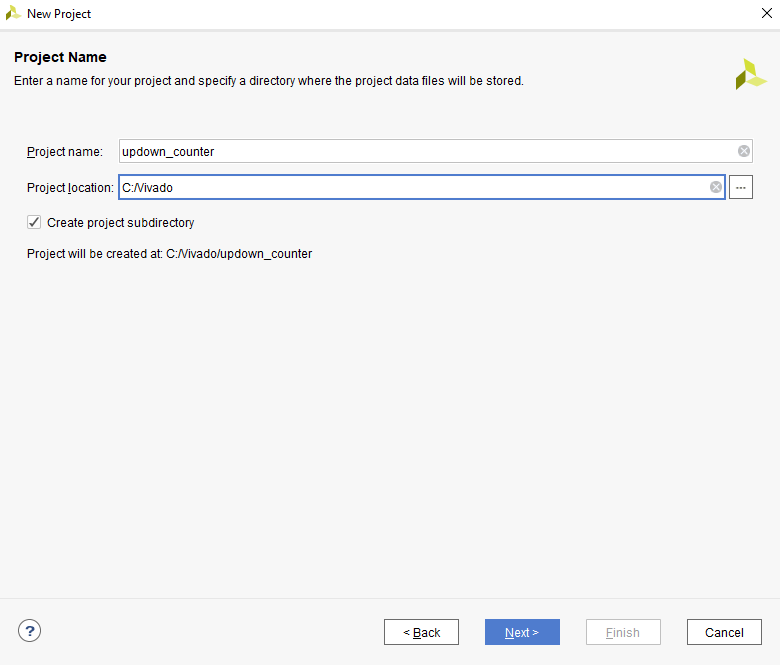
\includegraphics[width=0.5\linewidth]{img/program/2-project_name.png}
        \caption{Setting project name}
        \label{fig:2-project_name}
      \end{figure}

    \item Now that the project has a name and a place to save its files, the type of project needs to be selected. For this tutorial, we will create our 
      digital designs from scratch. Select "RTL Project" and check "Do not specify sources at this time" (see Fig. \ref{fig:3-project_type}). 
      We will create the source files later on this tutorial. Click "Next" to continue.
      \begin{figure}[h!]
        \centering
        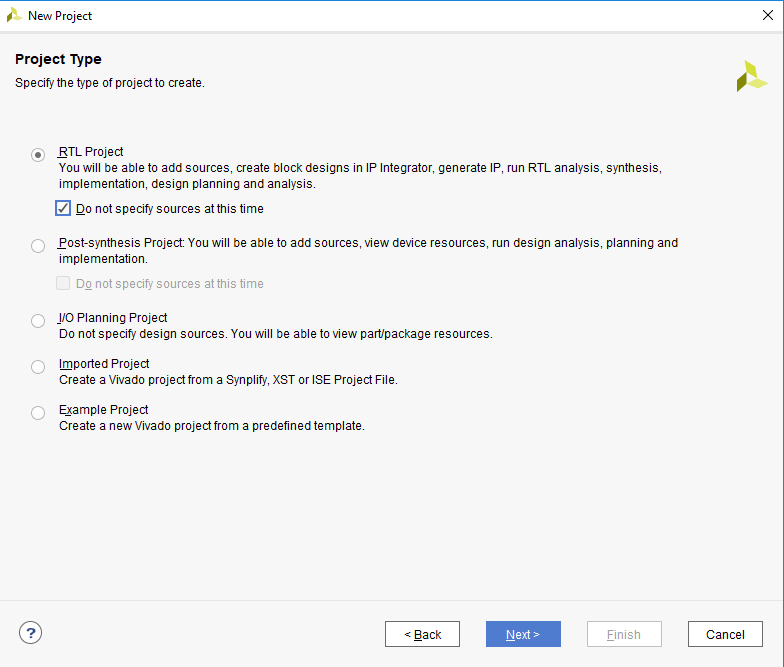
\includegraphics[width=0.5\linewidth]{img/program/3-project_type.png}
        \caption{Setting project type}
        \label{fig:3-project_type}
      \end{figure}

    \item Now, we will set the target device for our project (see Fig. \ref{fig:4-default_part}). Click the "Boards" tab at the top of the dialog box. Under "vendor", select "digilentinc.com" while 
      under "Name", select "Arty A7-35". Select the device from the search results and click "Next".
        \begin{figure}[h!]
          \centering
          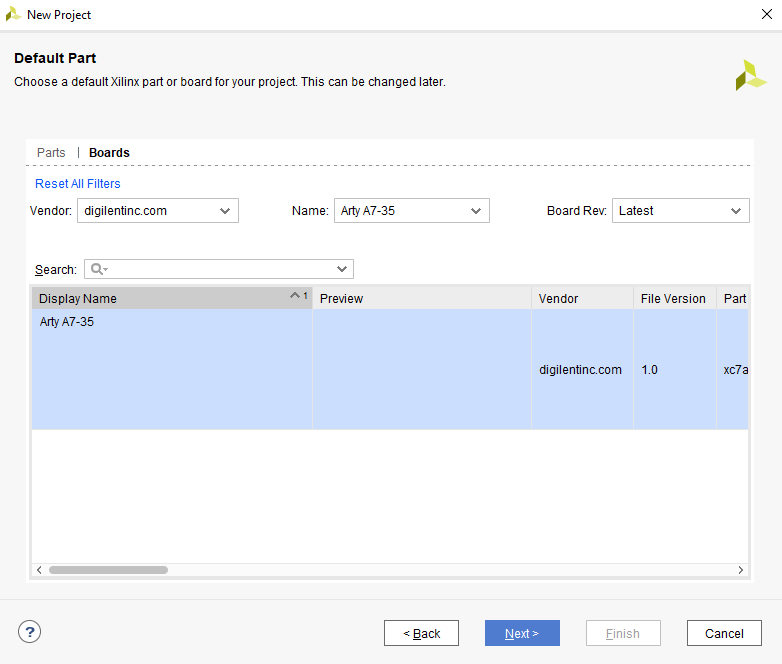
\includegraphics[width=0.5\linewidth]{img/program/4-default_part.png}
          \caption{Setting target device}
          \label{fig:4-default_part}
        \end{figure}

    \item The next window will show the summary of the project to be created. Verify that the project settings are correct (see Fig. \ref{fig:5-project_summary}).
      Click "Finish" to create the project.
        \begin{figure}[h!]
          \centering
          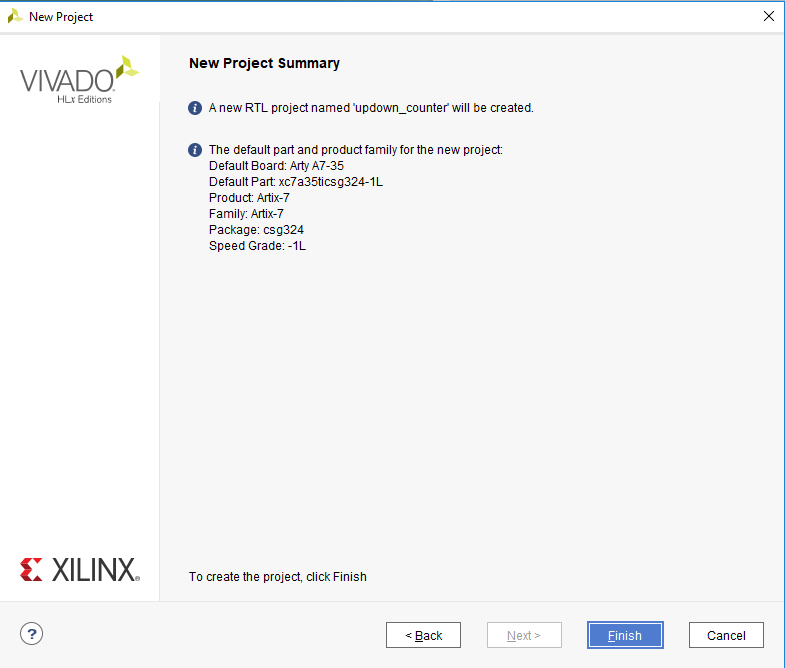
\includegraphics[width=0.5\linewidth]{img/program/5-project_summary.png}
          \caption{Project Summary}
          \label{fig:5-project_summary}
        \end{figure}

    \item After creating the project, the "Project Manager" window will open (see Fig. \ref{fig:6-project_window}).
        \begin{figure}[h!]
          \centering
          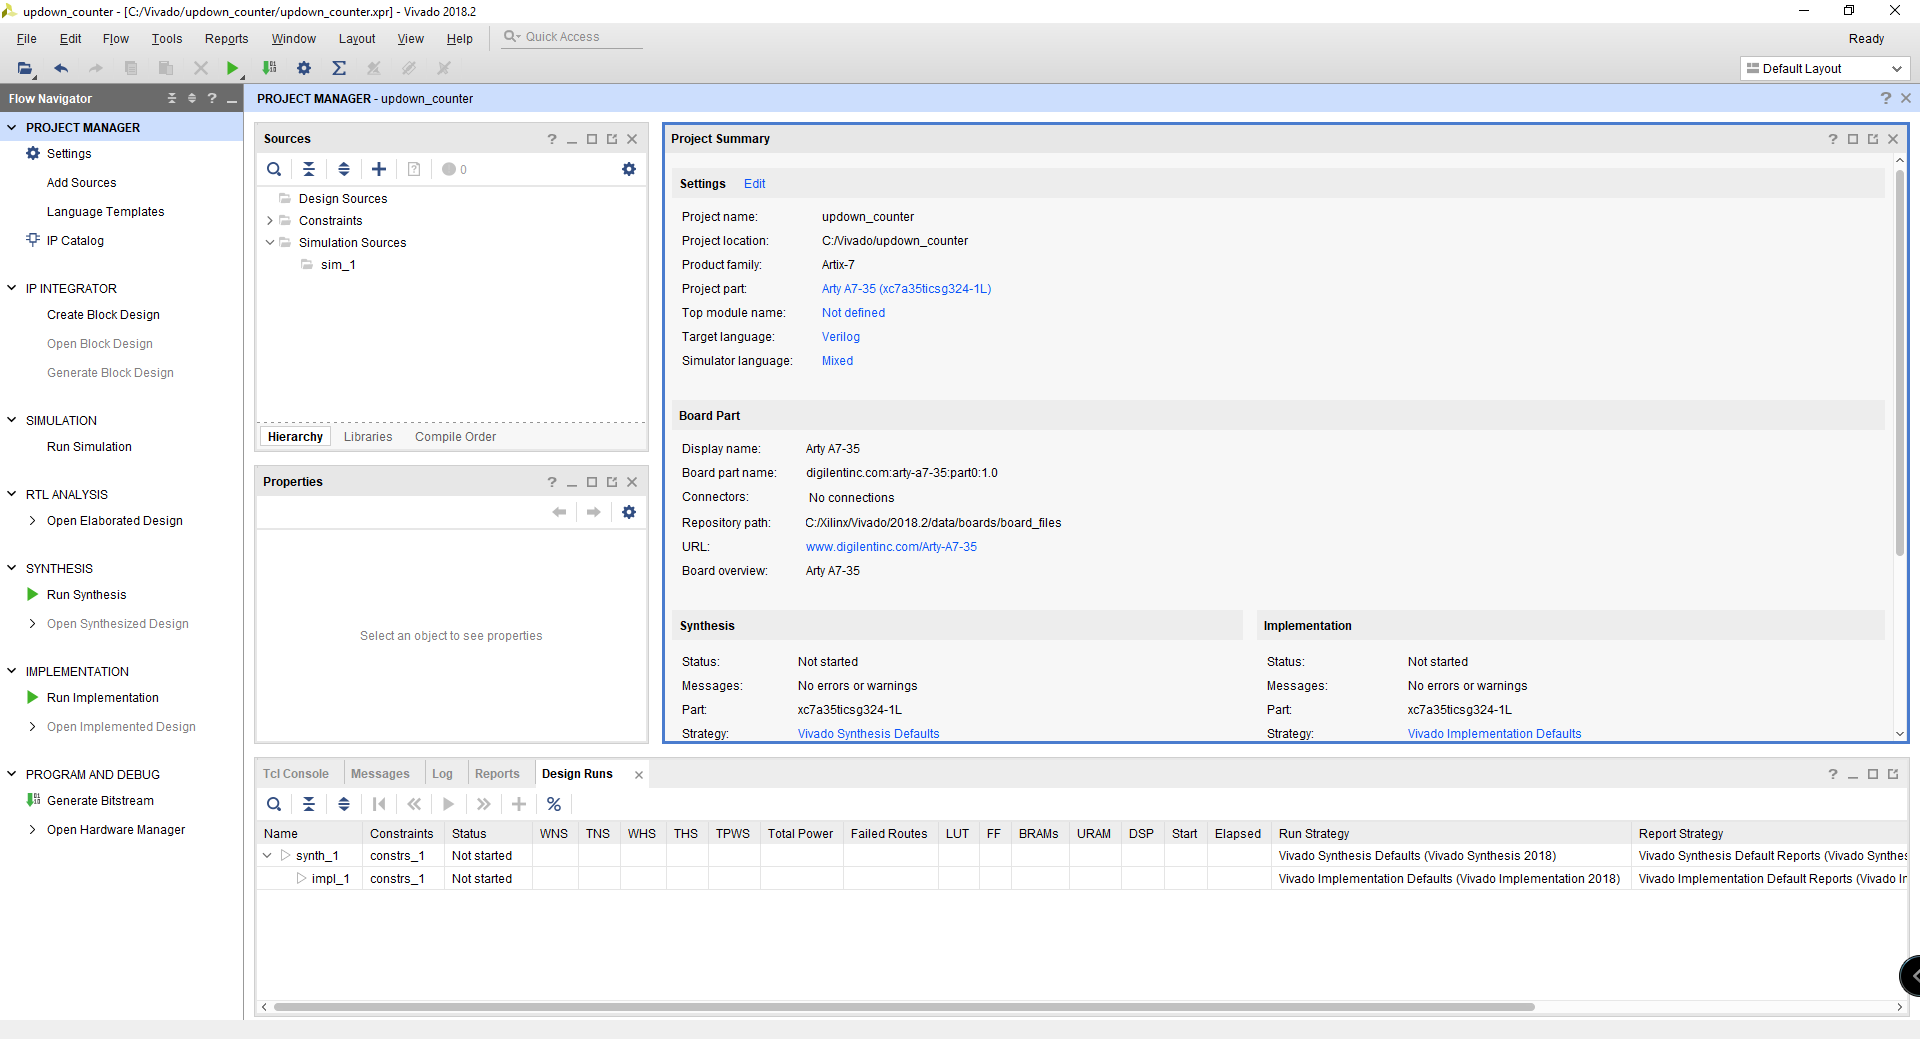
\includegraphics[width=\linewidth]{img/program/6-project_window.png}
          \caption{Project Manager window}
          \label{fig:6-project_window}
        \end{figure}
  \end{enumerate}

\newpage
\clearpage
\section*{Adding a constraint file}
  Now that we have created our project, we need to add a constraint file which will allow us to connect our HDL code with the physical pins 
  of the FPGA. For this tutorial, we will use the default Xilinx Design Constraint (XDC) file provided by Digilent which can be found on this repository
  (https://github.com/Digilent/digilent-xdc). The repository contains a list of XDC files targeted for each of the FPGA boards produced by Digilent. 
  For this tutorial, we will use the "Arty-A7-35-Master.xdc".
  \begin{enumerate}
    \item Under the "Flow Navigator" pane, click "Add Sources". This will open the "Add Sources" dialog box shown in Fig. \ref{fig:7-add_sources}.
    In the dialog box, select "Add or create constraints" and click "Next".
      \begin{figure}[h!]
        \centering
        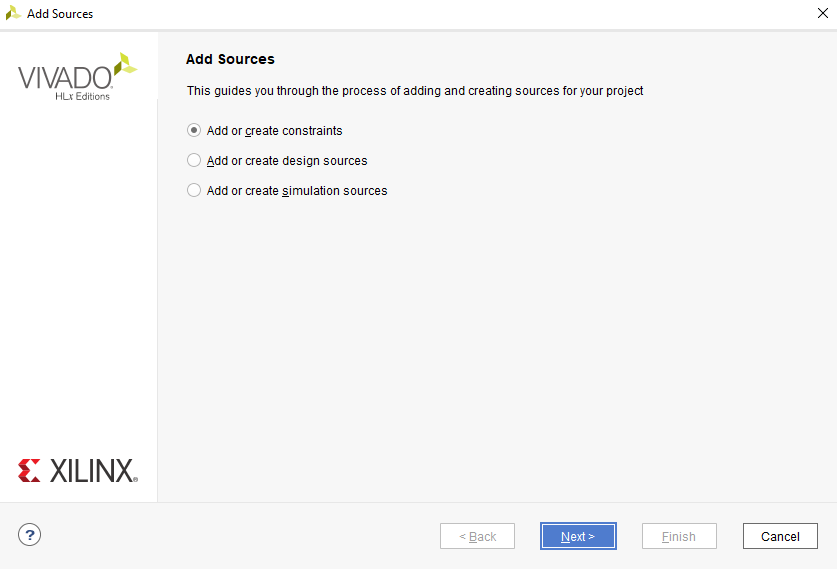
\includegraphics[width=0.5\linewidth]{img/program/7-add_sources.png}
        \caption{Add Sources Dialog Box}
        \label{fig:7-add_sources}
      \end{figure}

    \item In the "Add or Create Constraints" dialog box (see Fig. \ref{fig:8-add_constraint}), select "Add Files".
      \begin{figure}[h!]
        \centering
        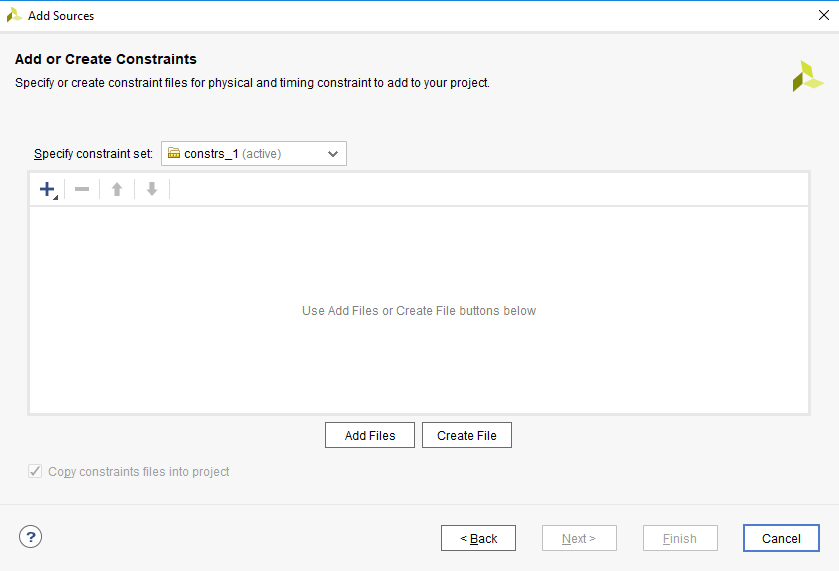
\includegraphics[width=0.5\linewidth]{img/program/8-add_constraint.png}
        \caption{Add Constraint File}
        \label{fig:8-add_constraint}
      \end{figure}

    \item The next step is to locate the XDC file to be added. Make sure to select "Arty-A7-35-Master.xdc" (see Fig. \ref{fig:9-locate_artyA7xdc}. 
    After selecting the XDC file, click "OK".
      \begin{figure}[h!]
        \centering
        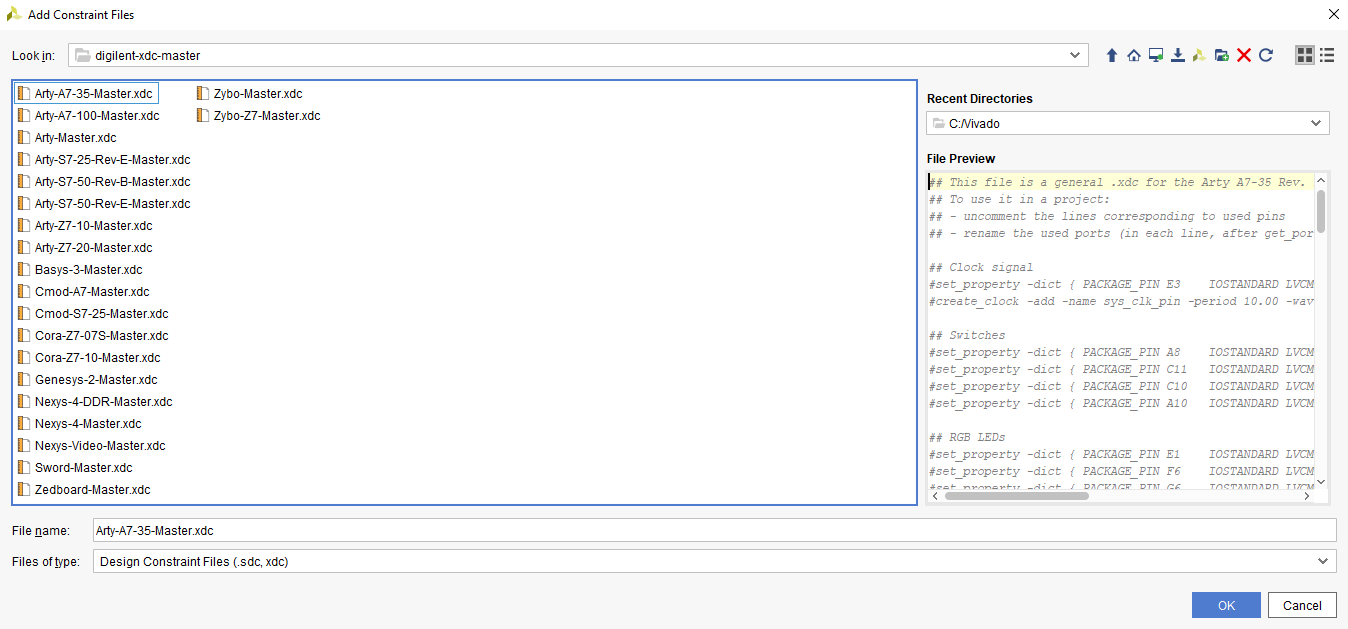
\includegraphics[width=\linewidth]{img/program/9-locate_artyA7xdc.png}
        \caption{Select Constraint File}
        \label{fig:9-locate_artyA7xdc}
      \end{figure}

    \item You will be prompted back to the "Add or Create Constraints" dialog box but now with the XDC file added (see Fig \ref{fig:10-add_constraint_done}). 
    Ensure that the "Copy constraints file into project" is checked. Click "Finish" to proceed.
      \begin{figure}[h!]
        \centering
        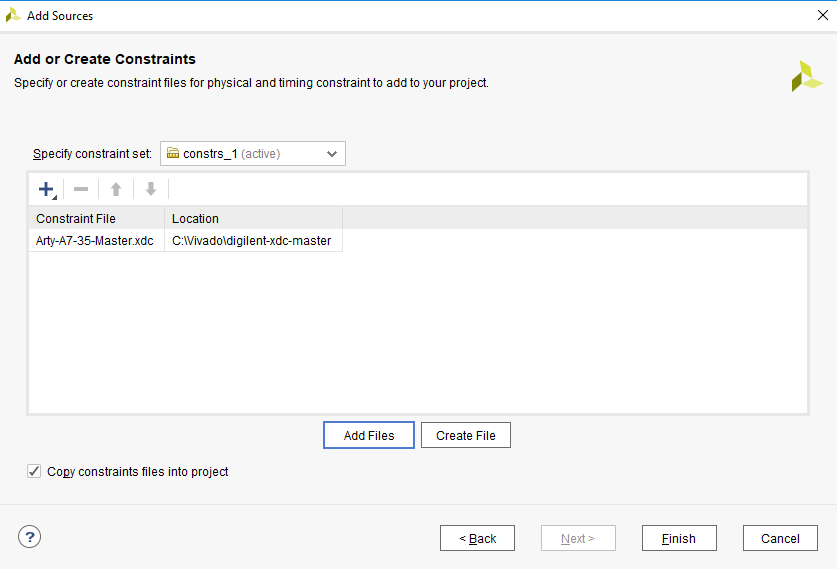
\includegraphics[width=0.5\linewidth]{img/program/10-add_constraint_done.png}
        \caption{XDC file added}
        \label{fig:10-add_constraint_done}
      \end{figure}

    \item After adding the constraint file, you will be prompted back to the "Project Manager" window. Notice that the added constraint file is listed under
      "Constraints - constr\_1" in the "Project Manager" window (see Fig. \ref{fig:11-project_window_constraint_added}).
      \begin{figure}[h!]
        \centering
        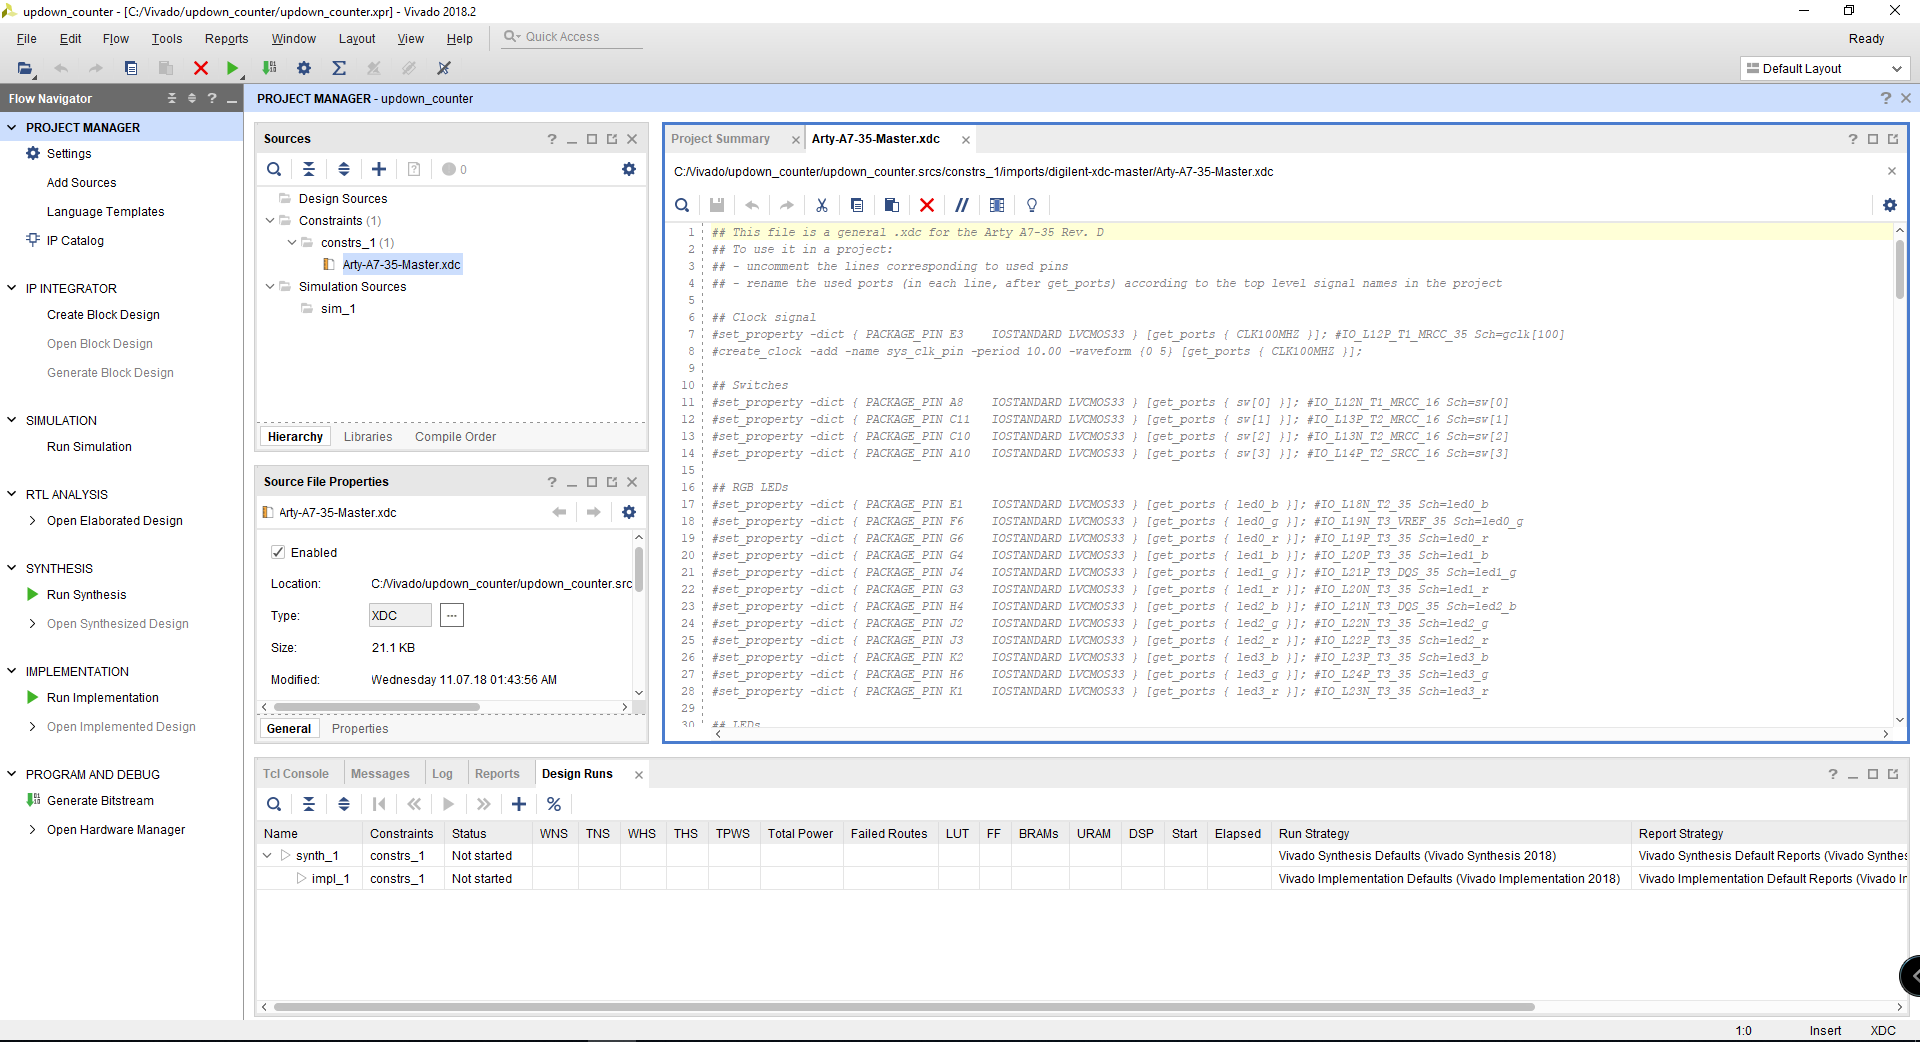
\includegraphics[width=\linewidth]{img/program/11-project_window_constraint_added.png}
        \caption{XDC file added}
        \label{fig:11-project_window_constraint_added}
      \end{figure}
  \end{enumerate}

\newpage
\clearpage
\section*{RTL Logic Design \& Behavioral Simulation}
  For this part of the tutorial, we will create our HDL source files for our intended digital design. 
  \begin{enumerate}
    \item To create a source file, click the "Add Sources" under the "Flow Navigator" pane. This will open the "Add Sources" dialog box (see Fig. \ref{fig:7-add_sources}). 
    Select "Add or create design sources" and click "Next".
    \item The "Add or Create Design Sources" will appear. You can add existing source files or create new ones. For this tutorial, we will be creating the HDL source files.
    In the dialog box, select "Create File" (see Fig. \ref{fig:12-add_source}). 
      \begin{figure}[h!]
        \centering
        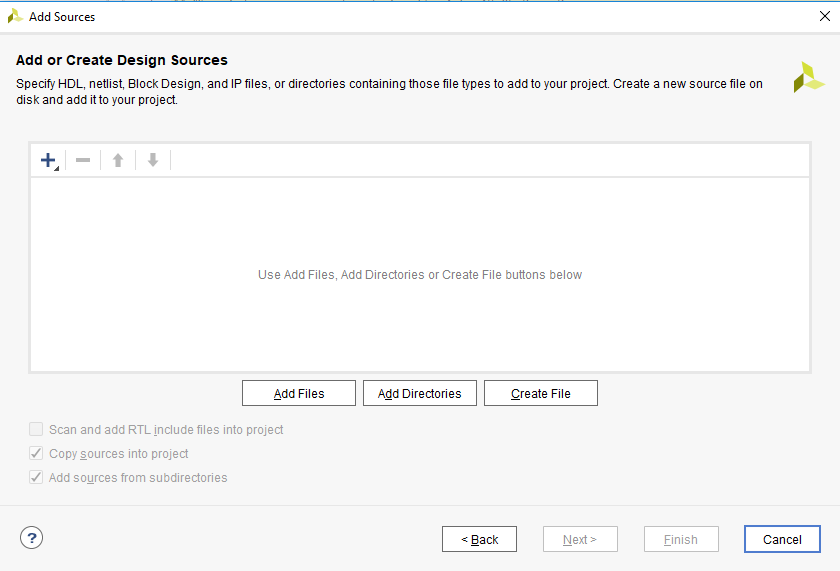
\includegraphics[width=0.5\linewidth]{img/program/12-add_source.png}
        \caption{Add source file}
        \label{fig:12-add_source}
      \end{figure}

    \item Now, you will be asked for the name and type of the new source file. Select "Verilog" for the file type and set the file name to "updown.v" 
    (see Fig. \ref{fig:13-create_source}). After that, click "OK" to continue.
      \begin{figure}[h!]
        \centering
        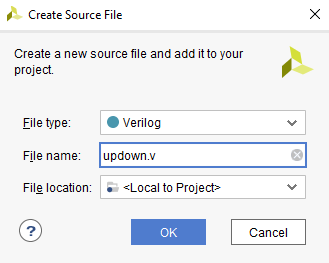
\includegraphics[width=0.4\linewidth]{img/program/13-create_source.png}
        \caption{Set file name and type of the source file}
        \label{fig:13-create_source}
      \end{figure}

    \item You will be prompted back to the "Add or Create Design Sources" with the new source file added (see Fig. \ref{fig:14-add_source_done}. 
    Click "Finish" to continue.
      \begin{figure}[h!]
        \centering
        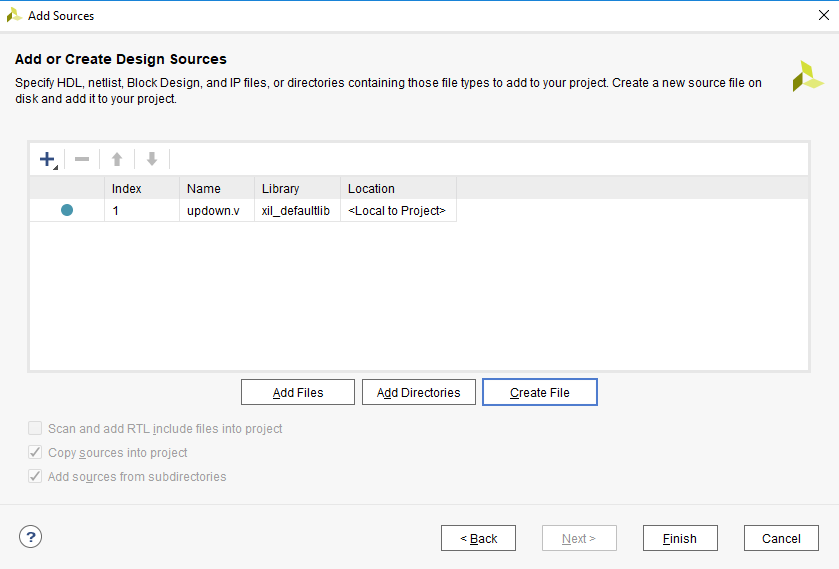
\includegraphics[width=0.5\linewidth]{img/program/14-add_source_done.png}
        \caption{Source file added}
        \label{fig:14-add_source_done}
      \end{figure}

    \item The next step is to define the input and output ports of our module. Add single bit ports clk, nrst, and dir as inputs. For the output port, 
    add a port named count with the bus option enabled, and set the most significant bit (MSB) to 3 and the least significant bit (LSB) to 0. Fig. 
    \ref{fig:15-define_module} shows the port declaration for the updown module. Note that you can still modify the module's ports after creating the source 
    file. This step just allows Vivado to auto-generate the port declaration part of the source code. Click "OK" to continue.
      \begin{figure}[h!]
        \centering
        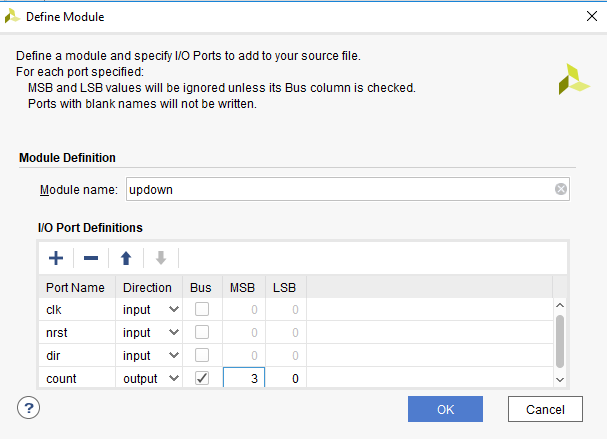
\includegraphics[width=0.5\linewidth]{img/program/15-define_module.png}
        \caption{Port declaration for the updown module}
        \label{fig:15-define_module}
      \end{figure}
    
    \item You will be prompted back to the "Project Manager" window. Notice that the created source file is listed under the "Design Sources" in the 
    "Project Manager" window (see Fig. \ref{fig:16-project_window_source_added}).
      \begin{figure}[h!]
        \centering
        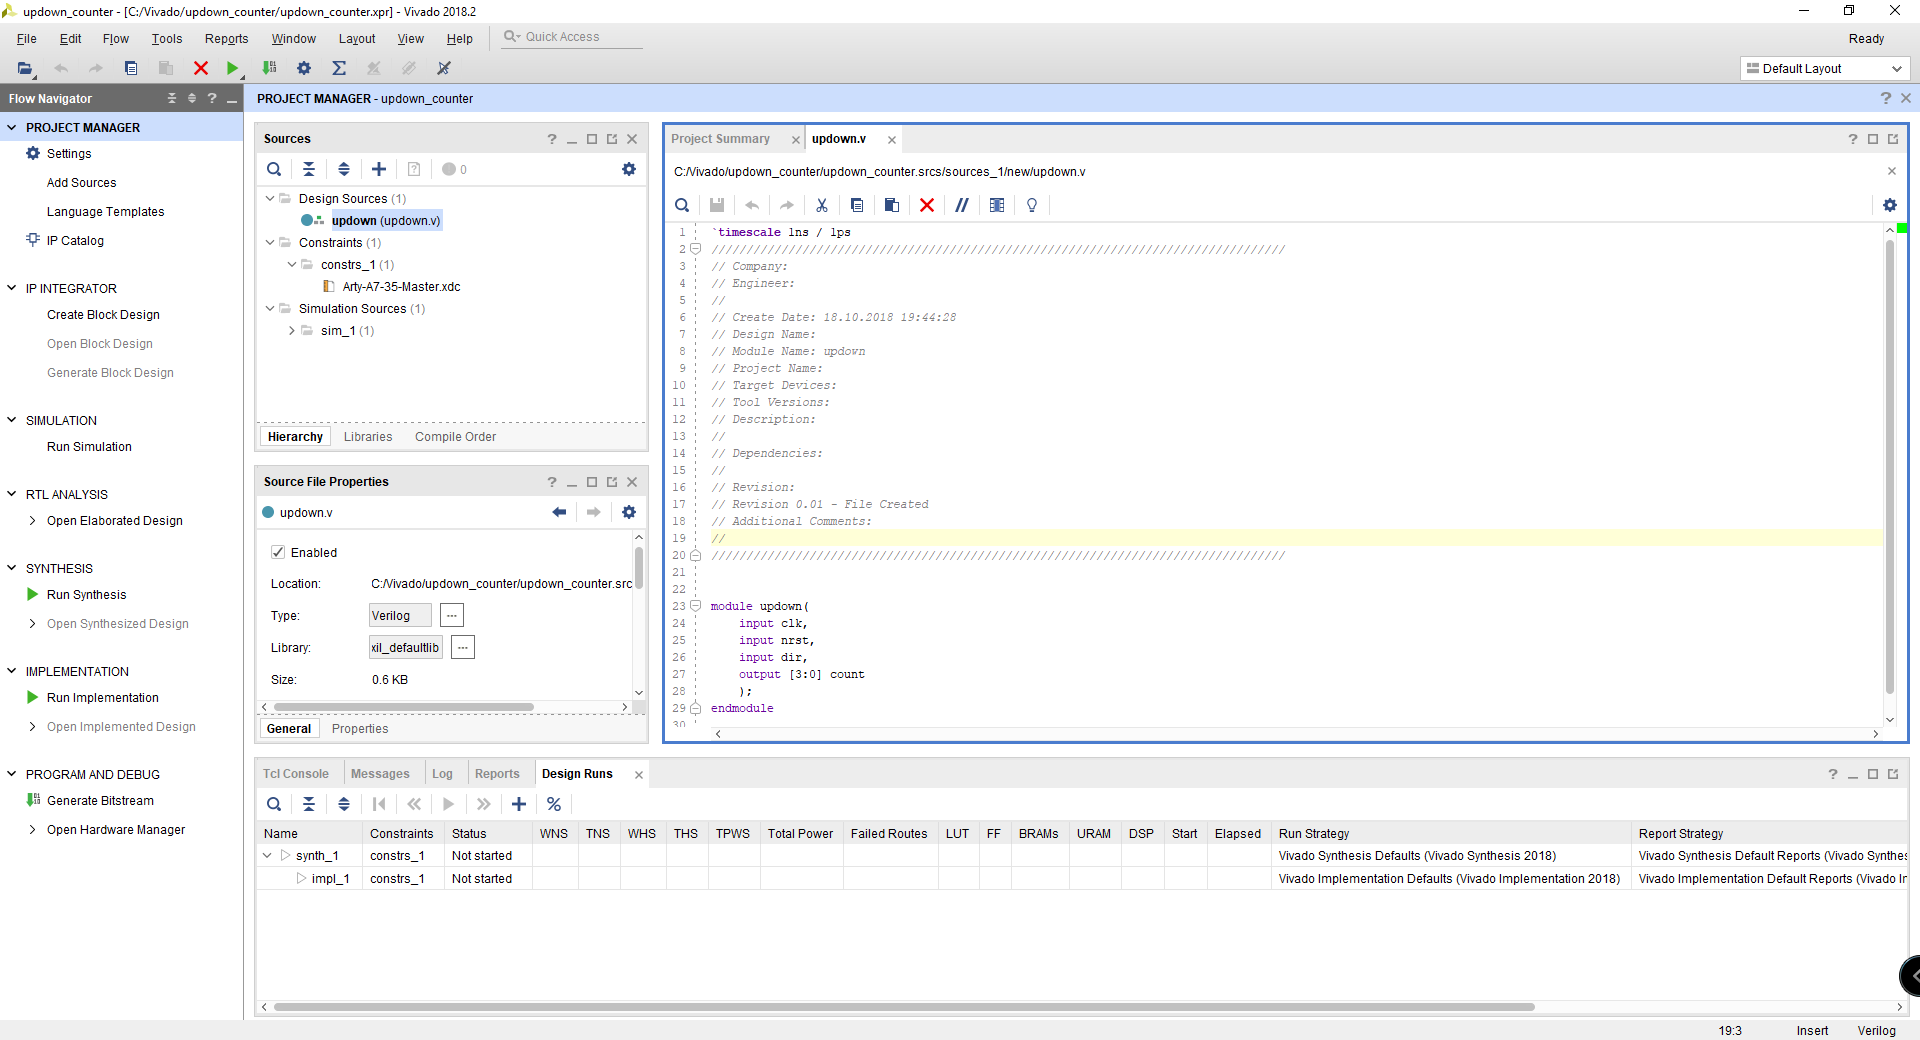
\includegraphics[width=\linewidth]{img/program/16-project_window_source_added.png}
        \caption{Source file added}
        \label{fig:16-project_window_source_added}
      \end{figure}

    \clearpage
    \item In the source pane, double-click the "updown.v" source file for editing. The contents of the source file will be shown in the workspace pane.
    Insert the following code shown in Code 1 on your source file. 
      \lstinputlisting[style=verilog, basicstyle=\small]{codes/updown.v}

    \item Now that we have defined the functionality of the updown module, the next step is to test whether our design is working or not. To do this,
    we need to create a simulation source file that will provide stimulus to the updown module. To create 
  \end{enumerate}
\end{document} 